% arara: pdflatex
% arara: pdflatex
% arara: pdflatex

% options:
% thesis=B bachelor's thesis
% thesis=M master's thesis
% czech thesis in Czech language
% slovak thesis in Slovak language
% english thesis in English language
% hidelinks remove colour boxes around hyperlinks

\documentclass[thesis=B,czech]{FITthesis}[2012/06/26]

\usepackage[utf8]{inputenc} % LaTeX source encoded as UTF-8

\usepackage{graphicx} %graphics files inclusion
% \usepackage{amsmath} %advanced maths
% \usepackage{amssymb} %additional math symbols

\usepackage{dirtree} %directory tree visualisation

% % list of acronyms
% \usepackage[acronym,nonumberlist,toc,numberedsection=autolabel]{glossaries}
% \iflanguage{czech}{\renewcommand*{\acronymname}{Seznam pou{\v z}it{\' y}ch zkratek}}{}
% \makeglossaries

\newcommand{\tg}{\mathop{\mathrm{tg}}} %cesky tangens
\newcommand{\cotg}{\mathop{\mathrm{cotg}}} %cesky cotangens

% % % % % % % % % % % % % % % % % % % % % % % % % % % % % % 
% ODTUD DAL VSE ZMENTE
% % % % % % % % % % % % % % % % % % % % % % % % % % % % % % 

\department{Katedra softwarového inženýrství}
\title{Webová aplikace pro online web scraping}
\authorGN{Jakub} %(křestní) jméno (jména) autora
\authorFN{Drahoš} %příjmení autora
\authorWithDegrees{Jakub Drahoš} %jméno autora včetně současných akademických titulů
\author{Jakub Drahoš} %jméno autora bez akademických titulů
\supervisor{Martin Podloucký}
\acknowledgements{Doplňte, máte-li komu a za co děkovat. V~opačném případě úplně odstraňte tento příkaz.}
\abstractCS{V~několika větách shrňte obsah a přínos této práce v~češtině. Po přečtení abstraktu by se čtenář měl mít čtenář dost informací pro rozhodnutí, zda chce Vaši práci číst.}
\abstractEN{Sem doplňte ekvivalent abstraktu Vaší práce v~angličtině.}
\placeForDeclarationOfAuthenticity{V~Praze}
\declarationOfAuthenticityOption{4} %volba Prohlášení (číslo 1-6)
\keywordsCS{Nahraďte seznamem klíčových slov v češtině oddělených čárkou.}
\keywordsEN{Nahraďte seznamem klíčových slov v angličtině oddělených čárkou.}
% \website{http://site.example/thesis} %volitelná URL práce, objeví se v tiráži - úplně odstraňte, nemáte-li URL práce

\begin{document}

% \newacronym{CVUT}{{\v C}VUT}{{\v C}esk{\' e} vysok{\' e} u{\v c}en{\' i} technick{\' e} v Praze}
% \newacronym{FIT}{FIT}{Fakulta informa{\v c}n{\' i}ch technologi{\' i}}

\begin{introduction}
	%sem napište úvod Vaší práce
\end{introduction}

% -----------------------------------------------------------------

\chapter{Cíl práce}

Cílem této práce je navržení a tvorba webové aplikace, která bude umož\v{n}ovat uživatelům vytáhnout požadovaná data z libovolné stránky v reálném čase bez jakékoli nutné znalosti programování.

Hlavním specifikem aplikace bude \emph{přehlednost a jednoduchost uživatelského rozhraní} -- je klíčové, aby bylo ovládání intuitivní, rychlé a jednoduché.

Naopak v rozsahu této práce není tvorba web crawlera ani žádného jiného podobného mechanismu, který by procházel danou oblast webu.

% -----------------------------------------------------------------

\chapter{Analýza a návrh}

\section{Co je to vlastně ten web scraping?}
\paragraph{Web sraping}
(nebo také \emph{web harvesting, web data extraction}) je technika získávání nejrůznějších dat z webových stránek. Nejčastěji se v tomto kontextu jedná o automatizovaný proces strojového zpracování a získávání dat, nicméně může jít i o manuální extrakci zadanou uživatelem skrze nějaký software (jako je tomu právě v našem případě). [citace z Wiki - web scraping]

Často se také v souvislosti s pojmem web scraping používá spojení \emph{web crawler} (nebo také \emph{bot, spider, spiderbot}). Jedná se o automatizovaný software, který systematicky prochází danou oblast webu a během toho extrahuje kýžená data. Jak již bylo řečeno v úvodu, touto částí web scrapingu se práce nebude zabývat.

\subsection{Krátce k historii}
Historie web scrapingu šahá k samým počátkům internetu (World Wide Web, 1989). Prvním webovým robotem, který byl vyvinut na MIT k měření velikosti webu, byl World Wide Web Wanderer (napsaný v jazyce Perl) z roku 1993. [citace z Wiki - World Wide Web Wanderer] 

O něco později, v roce 2000, se ve velkém začala používat webová APIs - lidé mohli konzumovat čistá data a scraping se tak stal o hodně jednodušším. 

Dalším milníkem v historii web scrapingu je rok 2004, kdy byla vydána knihovna pro parsování HTML a XML dokumentů Beautiful Soup pro programovací jazyk Python. Ta je do dnes považována za nejsofistikovanější a nejpokročilejší knihovnu pro web scraping.

Za zmínku stojí určitě i rok 2006, kdy je datován příchod vizuálního web scrapingu, tedy techniky, kdy uživatel jenom označí klikáním myší, z kterých oblastí webové stránky chce vytáhnout data. Tímto se otevřely dveře web scrapingu pro všechny. [citace z https://www.octoparse.com/blog/web-scraping-introduction]

\subsection{Techniky}
Technik web scrapingu existuje mnoho, podívejme se alespo\v{n} na některé z nich:
\begin{itemize}
	\item Vyhledávání na základě textové shody -- např. pomocí UNIX nástroje grep nebo regulárních výrazů
	\item HTML parsování -- základní a stále ještě nejpoužívanější technika extrakce dat. Informace jednoduše získáváme z HTML elementů, popř. pomocí tříd nebo id
	\item Počítačové vidění, strojové učení, zapojení umělé inteligence -- snaha napodobit způsob, jakým vidí a zpracovává webovou stránku člověk, něco podobného zkouší např. \emph{Diffbot}
	\item Ruční vyhledávání -- může se ukázat, že někdy je to tou nejsnažší a nejrychlejší alternativou
\end{itemize}

\subsection{Využití web scrapingu}
Podob pro uplatnění scrapování dat z webu je nespočet, a to obzvláš\v{t} v dnešní době, kdy jsme přímo zaplaveni daty (pohybujeme se v řádech Zettabajtů -- $1024^{7}$ B [citace z https://www.nodegraph.se/big-data-facts/]). Mezi ty hlavní patří:
\begin{itemize}
	\item Získání kontaktních informací (např. e-mail) pro marketingové účely
	\item Indexování webových stránek
	\item Data mining - proces hledání vzorců ve velkých datových setech [odkaz na Wiki]
	\item Monitorování různých proměných (např. sledování cen nebo hodnocení produktů)
	\item Recyklace již někdy použitých dat za účelem vytváření \uv{nového} obsahu
	\item Analýza a zpracování dat k výzkumným účelům
\end{itemize}

\subsection{Je to vlastně legální?}


\newpage
\section{Analýza konkurence}
První skupinou, na kterou můžeme při hledání na internetu narazit, jsou společnosti, které nabízejí zákazníkům kompletní péči v rámci extrakce dat. Cílí především na velké korporace, jimž postaví scrapovací nástroj přesně na míru, který poté také hostují a spravují. Zákazník tedy dostane data a o nic víc se již nemusí starat. Jako příklad můžeme jmenovat třeba \emph{ContentGrabber, Mozenda} a další.

Pro nás mnohem relevantnější kategorií je konkurenční nabídku nástrojů poskytujících uživatelům rozhraní k web scrapingu. Budeme se zaměřovat pouze na takové nástroje, které nevyžadují jakoukoli znalost programování -- tedy žádné knihovny, API a nástroje pro budování vlastních scraperů.

Mezi ty největší představitele patří \emph{ParseHub, Octoparse, WebScraper, Data Scraper} a \emph{Dexi.io}. Čtyři z nich jsou volně dostupné nástroje (které mají ale velmi omezenou funkcionalitu a pokročilejší operace se odemknou až s určitým platebním plánem) a jeden poskytuje bezplatně pouze 7 denní zkušební verzi.

Předtím, než začneme jednotlivé nástroje porovnávat, musíme si určit nějaká kritéria, podle kterých budeme hodnotit kvalitu daného nástroje. Především nám půjde o jednoduchost používání, celkovou přehlednost a rychlost, se kterou se uživatel dostane k požadovaným datům. Také nás bude zajímat způsob výběru dat, možnosti exportu získaných dat, jak aplikace sama dokáže seznámit uživatele s používáním a také, v jaké formě se nástroj vůbec používá a jestli něčím vybočuje (a\v{t} už v pozitivním nebo negativním smyslu). 

Poj\v{d}me se tedy na některé nástroje podívat blíže:

\subsection{ParseHub}
\begin{figure}[h]
	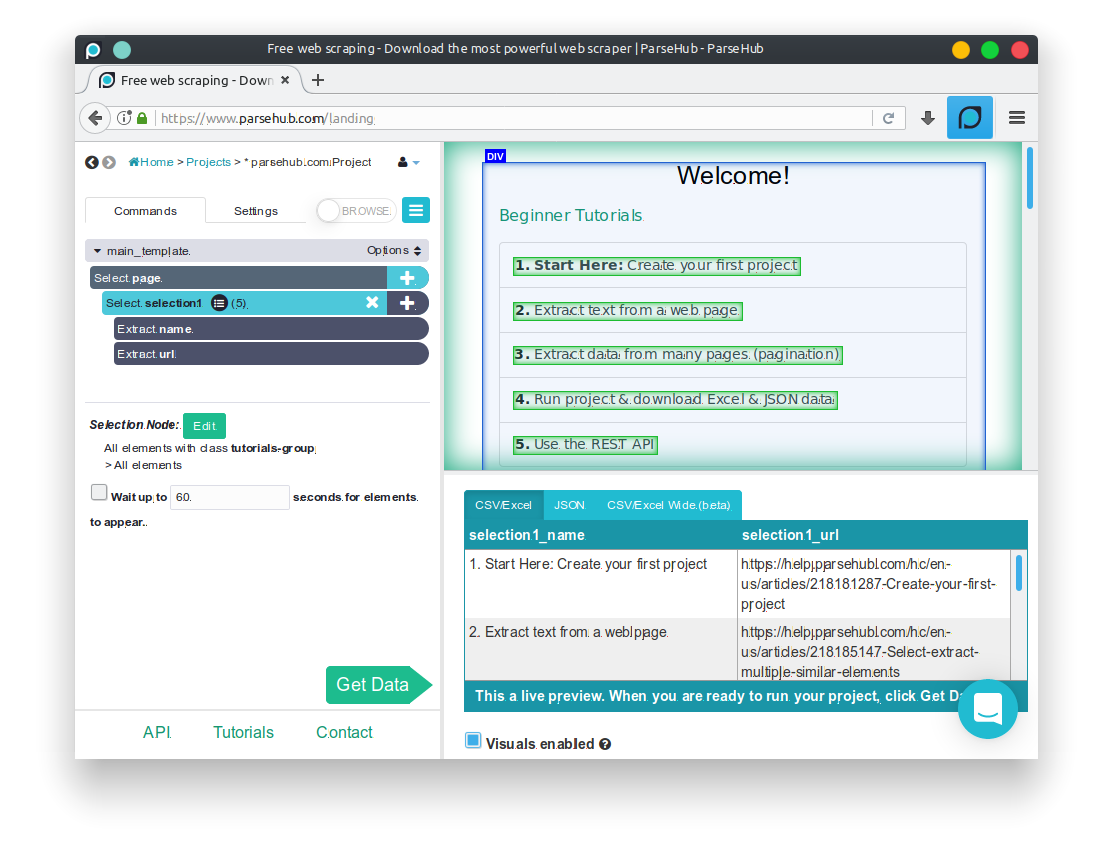
\includegraphics[width=\linewidth]{images/ParseHub.png}
	\caption{ParseHub}
	\label{fig:parseHub}
\end{figure}

\textbf{Výhody:}
\begin{itemize}
	\item Výběr dat jak pomocí klikání (inteligentní hledání vzorců/podobností na základě prvních dvou kliknutí), tak pomocí XPath, regulárních výrazů nebo CSS selektorů
	\item Aplikace obsahuje interaktivní tutoriál, který na jednoduchých příkladech ukáže, jak s nástrojem zacházet
	\item Možnost získání dat různými formami - přes API, jako CSV/Excel, do GoogleSheets nebo do Tableau
	\item Různé módy kliknutí (výběr, relativní výběr, kliknutí), zooming in/out na HTML elementy -- když se uživatel netrefí (nebo ani trefit nemůže) přesně na požadovaný element, lze na něj lehce přejít pomocí této funkce
	\item Automatická rotace IP adresy (tedy nedochází k blokování ze strany serveru)
\end{itemize}

\textbf{Nevýhody:}
\begin{itemize}
	\item Nutnost stažení aplikace (ale je zde podpora pro Windows, Linux i Mac)
	\item Aplikace je celkem těžkopádná, nemá moc přívětivé uživatelské rozhraní, ovládání působí nepřehledně a přehlceně -- na uživatele se vyvalí hodně informací a možností najednou
\end{itemize}


\newpage
\subsection{Octoparse}
\begin{figure}[h]
	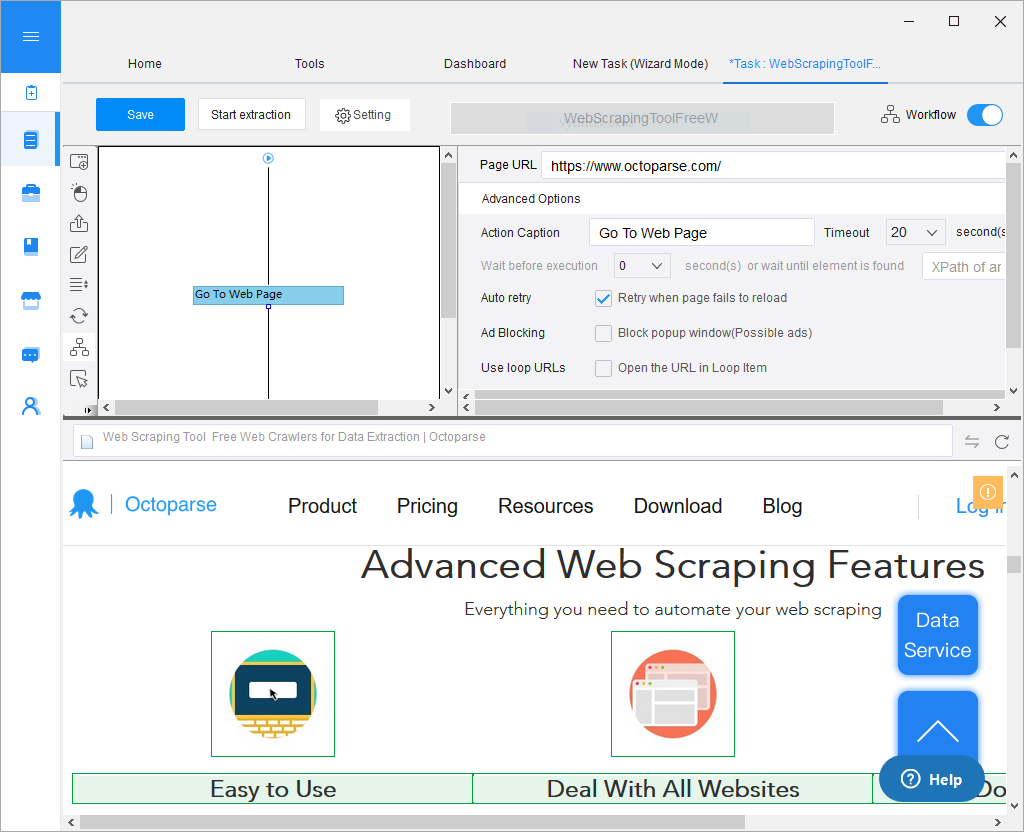
\includegraphics[width=\linewidth]{images/Octoparse.png}
	\caption{Octoparse}
	\label{fig:octoparse}
\end{figure}

\textbf{Výhody:}
\begin{itemize}
	\item Výběr dat jak pomocí klikání (inteligentní hledání vzorců/podobností na základě prvních dvou kliknutí), tak pomocí XPath nebo regulárních výrazů
	\item Nástroj obsahuje předpřipravené šablony, které mohou velmi urychlit práci
	\item Pestrá paleta možností (branch judgment, tvoření smyček apod.) -- dá se vytvořit téměř jakákoli logika procházení webu a extrakce dat
	\item Lehký způsob, jak scrapování automatizovat
	\item Možnost řídit tasky přes API (a získávat tak data taktéž přes API). Data jdou nahrát rovnou i do lokální databáze\\\\
\end{itemize}

\textbf{Nevýhody:}
\begin{itemize}
	\item Nutnost stažení aplikace (která je navíc pouze pro Windows)
	\item Těžkopádné a pomalé ovládání, neintuitivní rozhraní
	\item Tutoriál je v podstatě nic neříkající
	\item Předpřipravených šablon je jenom pár a jsou velmi konkrétní
\end{itemize}


\newpage
\subsection{WebScaper}
\begin{figure}[h]
	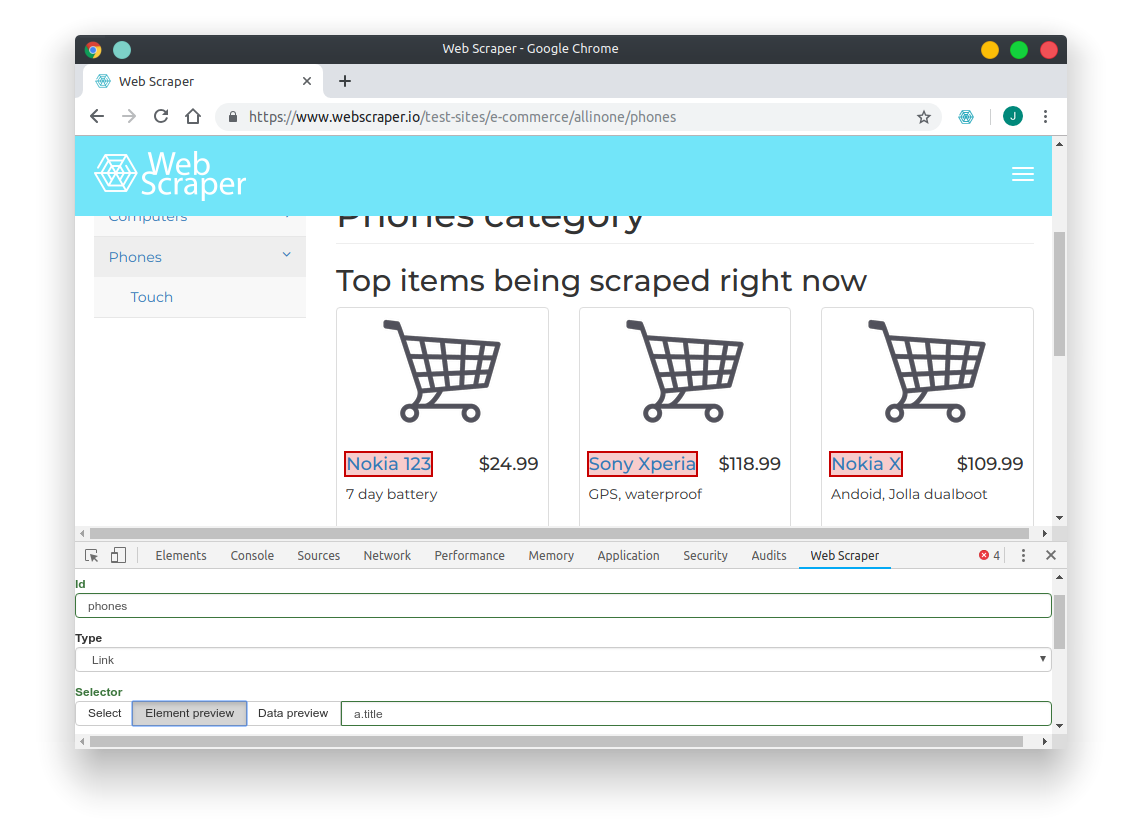
\includegraphics[width=\linewidth]{images/WebScraper.png}
	\caption{WebScraper}
	\label{fig:webScraper}
\end{figure}

\textbf{Výhody:}
\begin{itemize}
	\item Jednoduchá instalace (jedná se pouze o rozšíření do prohlížeče Google Chrome). Nastavování probíhá skrze vývojářskou konzoli
	\item Výběr dat pomocí klikání (inteligentní hledání vzorců/podobností na základě prvních dvou kliknutí)
	\item Tutoriály jsou formou videí -- jednoduché, rychlé a naprosto postačující
	\item Různé typy elementů, které vybíráme (text, odkaz, scroll down), takže lze celkem snadno prolézt celou stránku
	\item Možnost získání dat různými formami - přes API, jako CSV/Excel nebo do Dropboxu
	\item Klávesové zkratky při výběru elementů velmi usnad\v{n}ují práci
	\item Možnost využít jejich cloud k automatizaci celého procesu
	\item Oproti konkurenci nabízí přehledné rozhraní, rychlé a jednoduché používání
\end{itemize}

\textbf{Nevýhody:}
\begin{itemize}
	\item Nutnost používat Google Chrome, což pro některé uživatele může být překážka
	\item Nelze vyhledávat podle klíčových slov ani podle HTML nebo CSS, tudíž všechno se musí poctivě naklikat
\end{itemize}


\newpage
\subsection{Dexi.io}
\begin{figure}[h!]
	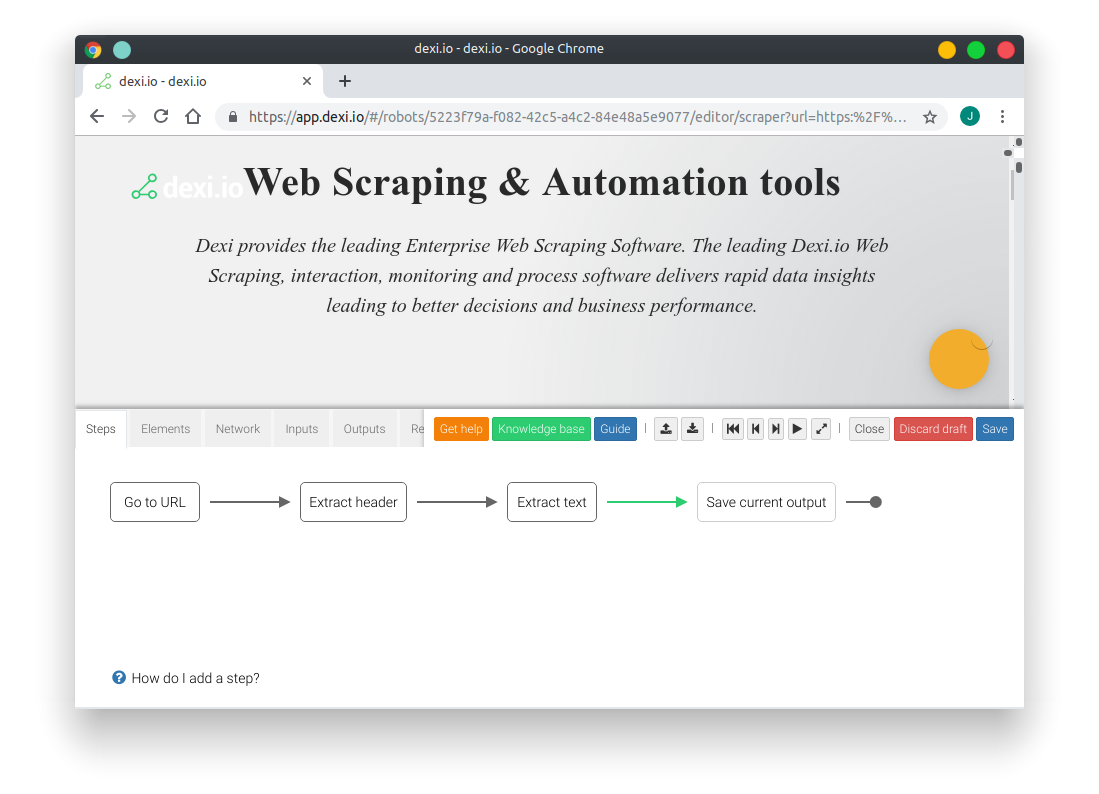
\includegraphics[width=\linewidth]{images/Dexiio.png}
	\caption{Dexi.io}
	\label{fig:dexi.io}
\end{figure}

\textbf{Výhody:}
\begin{itemize}
	\item Bez nutnosti stahování aplikace -- vše se ovládá přes webové rozhraní
	\item Výběr dat jak pomocí klikání (inteligentní hledání vzorců/podobností na základě prvních dvou kliknutí), tak pomocí HTML, CSS nebo textové shody
	\item Hodně návodů dostupných na stránkách, interaktivní rádce přímo při scrapování
	\item Všechny možné druhy kliknutí, takže lze lehce prolézt celou stránku
	\item Možnost exportovat data do CSV, JSON, XLS, získat přes API, poslat do Google Drive, Google Sheets nebo Amazon S3
	\item Různé módy aplikace -- scraping, crawler, pipes (skládání menších scrape botů) a autobot (extrahování z více stránek najednou se stejným rozložením). Možnost takto automatizovat celý proces.
	\item Různé addony (např. na obcházení Captchy)
\end{itemize}

\textbf{Nevýhody:}
\begin{itemize}
	\item Široká nabídka možností a tak chvílí trvá, než se člověk zorientuje
	\item Placený nástroj, zadarmo je dostupná pouze týdenní zkušební verze
	\item Úvodní tutoriál je velmi strohý a žádné velké seznámení s nástrojem se nekoná
\end{itemize}


\newpage
\subsection{Data Scraper}
\begin{figure}[h]
	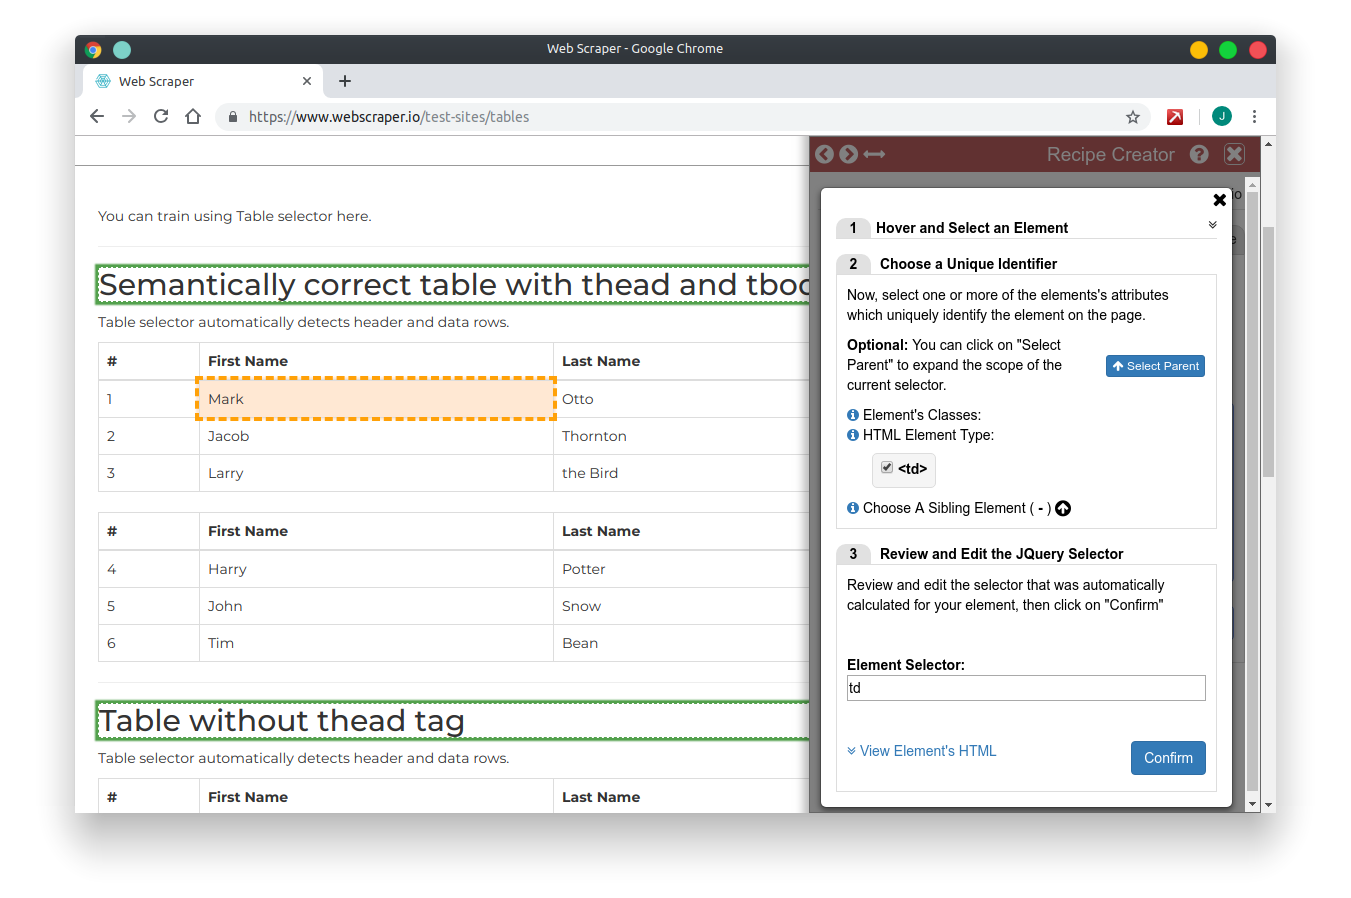
\includegraphics[width=\linewidth]{images/DataScraper.png}
	\caption{Data Scraper}
	\label{fig:dataScraper}
\end{figure}
\textbf{Výhody:}
\begin{itemize}
	\item Jednoduchá instalace (jedná se pouze o rozšíření do prohlížeče Google Chrome).
	\item Velmi jednoduché ovládání a přehledné rozhraní
	\item Výběr dat probíhá pomocí klikání. Skvělé je, že klikáním se utváří JQuery selektor, který si uživatel může podle svého upravit a doladit tak drobné detaily, které by jinak nutně zahltily uživatelské rozhraní. Tedy je možné vyhledávat i podle HTML tagů, id, CSS selektorů -- zkrátka vše, co umí klasické JQuery
	\item Různé druhy kliknutí, možnost spustit na stránce libovolný JavaScriptový kód v rámci scrapování
\end{itemize}

\textbf{Nevýhody:}
\begin{itemize}
	\item Nutnost používat Google Chrome, což pro některé uživatele může být překážka
	\item Oproti ostatním nástrojům se může zdát velmi chudý na různé vychytávky
\end{itemize}


% -----------------------------------------------------------------

\chapter{Realizace}

% -----------------------------------------------------------------

\begin{conclusion}
	%sem napište závěr Vaší práce
\end{conclusion}

\bibliographystyle{csn690}
\bibliography{mybibliographyfile}

\appendix

% -----------------------------------------------------------------

\chapter{Seznam použitých zkratek}
% \printglossaries
\begin{description}
	\item[GUI] Graphical user interface
	\item[XML] Extensible markup language
\end{description}


% % % % % % % % % % % % % % % % % % % % % % % % % % % % 
% % Tuto kapitolu z výsledné práce ODSTRAŇTE.
% % % % % % % % % % % % % % % % % % % % % % % % % % % % 
% 
% \chapter{Návod k~použití této šablony}
% 
% Tento dokument slouží jako základ pro napsání závěrečné práce na Fakultě informačních technologií ČVUT v~Praze.
% 
% \section{Výběr základu}
% 
% Vyberte si šablonu podle druhu práce (bakalářská, diplomová), jazyka (čeština, angličtina) a kódování (ASCII, \mbox{UTF-8}, \mbox{ISO-8859-2} neboli latin2 a nebo \mbox{Windows-1250}). 
% 
% V~české variantě naleznete šablony v~souborech pojmenovaných ve formátu práce\_kódování.tex. Typ může být:
% \begin{description}
% 	\item[BP] bakalářská práce,
% 	\item[DP] diplomová (magisterská) práce.
% \end{description}
% Kódování, ve kterém chcete psát, může být:
% \begin{description}
% 	\item[UTF-8] kódování Unicode,
% 	\item[ISO-8859-2] latin2,
% 	\item[Windows-1250] znaková sada 1250 Windows.
% \end{description}
% V~případě nejistoty ohledně kódování doporučujeme následující postup:
% \begin{enumerate}
% 	\item Otevřete šablony pro kódování UTF-8 v~editoru prostého textu, který chcete pro psaní práce použít -- pokud můžete texty s~diakritikou normálně přečíst, použijte tuto šablonu.
% 	\item V~opačném případě postupujte dále podle toho, jaký operační systém používáte:
% 	\begin{itemize}
% 		\item v~případě Windows použijte šablonu pro kódování \mbox{Windows-1250},
% 		\item jinak zkuste použít šablonu pro kódování \mbox{ISO-8859-2}.
% 	\end{itemize}
% \end{enumerate}
% 
% 
% V~anglické variantě jsou šablony pojmenované podle typu práce, možnosti jsou:
% \begin{description}
% 	\item[bachelors] bakalářská práce,
% 	\item[masters] diplomová (magisterská) práce.
% \end{description}
% 
% \section{Použití šablony}
% 
% Šablona je určena pro zpracování systémem \LaTeXe{}. Text je možné psát v~textovém editoru jako prostý text, lze však také využít specializovaný editor pro \LaTeX{}, např. Kile.
% 
% Pro získání tisknutelného výstupu z~takto vytvořeného souboru použijte příkaz \verb|pdflatex|, kterému předáte cestu k~souboru jako parametr. Vhodný editor pro \LaTeX{} toto udělá za Vás. \verb|pdfcslatex| ani \verb|cslatex| \emph{nebudou} s~těmito šablonami fungovat.
% 
% Více informací o~použití systému \LaTeX{} najdete např. v~\cite{wikilatex}.
% 
% \subsection{Typografie}
% 
% Při psaní dodržujte typografické konvence zvoleného jazyka. České \uv{uvozovky} zapisujte použitím příkazu \verb|\uv|, kterému v~parametru předáte text, jenž má být v~uvozovkách. Anglické otevírací uvozovky se v~\LaTeX{}u zadávají jako dva zpětné apostrofy, uzavírací uvozovky jako dva apostrofy. Často chybně uváděný symbol "{} (palce) nemá s~uvozovkami nic společného.
% 
% Dále je třeba zabránit zalomení řádky mezi některými slovy, v~češtině např. za jednopísmennými předložkami a spojkami (vyjma \uv{a}). To docílíte vložením pružné nezalomitelné mezery -- znakem \texttt{\textasciitilde}. V~tomto případě to není třeba dělat ručně, lze použít program \verb|vlna|.
% 
% Více o~typografii viz \cite{kobltypo}.
% 
% \subsection{Obrázky}
% 
% Pro umožnění vkládání obrázků je vhodné použít balíček \verb|graphicx|, samotné vložení se provede příkazem \verb|\includegraphics|. Takto je možné vkládat obrázky ve formátu PDF, PNG a JPEG jestliže používáte pdf\LaTeX{} nebo ve formátu EPS jestliže používáte \LaTeX{}. Doporučujeme preferovat vektorové obrázky před rastrovými (vyjma fotografií).
% 
% \subsubsection{Získání vhodného formátu}
% 
% Pro získání vektorových formátů PDF nebo EPS z~jiných lze použít některý z~vektorových grafických editorů. Pro převod rastrového obrázku na vektorový lze použít rasterizaci, kterou mnohé editory zvládají (např. Inkscape). Pro konverze lze použít též nástroje pro dávkové zpracování běžně dodávané s~\LaTeX{}em, např. \verb|epstopdf|.
% 
% \subsubsection{Plovoucí prostředí}
% 
% Příkazem \verb|\includegraphics| lze obrázky vkládat přímo, doporučujeme však použít plovoucí prostředí, konkrétně \verb|figure|. Například obrázek \ref{fig:float} byl vložen tímto způsobem. Vůbec přitom nevadí, když je obrázek umístěn jinde, než bylo původně zamýšleno -- je tomu tak hlavně kvůli dodržení typografických konvencí. Namísto vynucování konkrétní pozice obrázku doporučujeme používat odkazování z~textu (dvojice příkazů \verb|\label| a \verb|\ref|).
% 
% \begin{figure}\centering
% 	
\includegraphics[width=0.5\textwidth, angle=30]{cvut-logo-bw}
% 	\caption[Příklad obrázku]{Ukázkový obrázek v~plovoucím prostředí}\label{fig:float}
% \end{figure}
% 
% \subsubsection{Verze obrázků}
% 
% % Gnuplot BW i barevně
% Může se hodit mít více verzí stejného obrázku, např. pro barevný či černobílý tisk a nebo pro prezentaci. S~pomocí některých nástrojů na generování grafiky je to snadné.
% 
% Máte-li například graf vytvořený v programu Gnuplot, můžete jeho černobílou variantu (viz obr. \ref{fig:gnuplot-bw}) vytvořit parametrem \verb|monochrome dashed| příkazu \verb|set term|. Barevnou variantu (viz obr. \ref{fig:gnuplot-col}) vhodnou na prezentace lze vytvořit parametrem \verb|colour solid|.
% 
% \begin{figure}\centering
% 	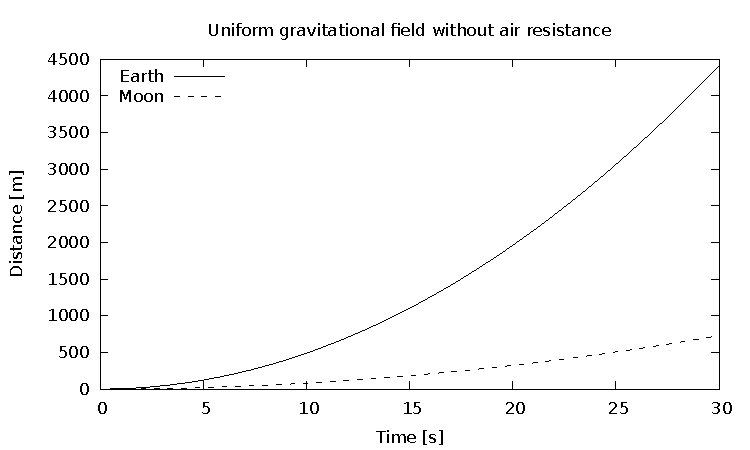
\includegraphics{gnuplot-bw}
% 	\caption{Černobílá varianta obrázku generovaného programem Gnuplot}\label{fig:gnuplot-bw}
% \end{figure}
% 
% \begin{figure}\centering
% 	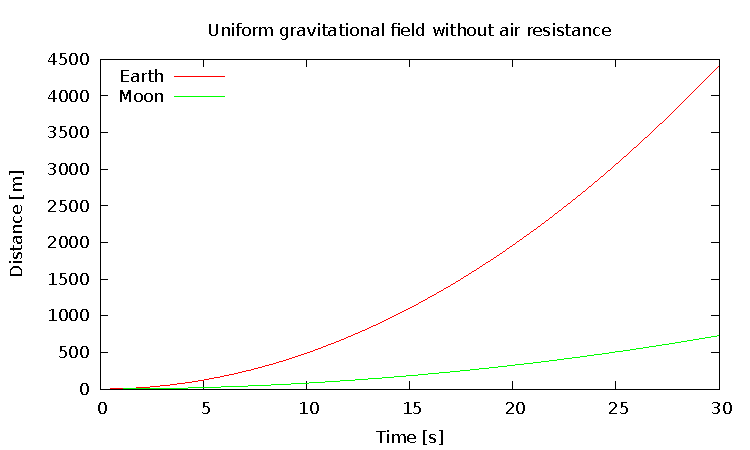
\includegraphics{gnuplot-col}
% 	\caption{Barevná varianta obrázku generovaného programem Gnuplot}\label{fig:gnuplot-col}
% \end{figure}
% 
% 
% \subsection{Tabulky}
% 
% Tabulky lze zadávat různě, např. v~prostředí \verb|tabular|, avšak pro jejich vkládání platí to samé, co pro obrázky -- použijte plovoucí prostředí, v~tomto případě \verb|table|. Například tabulka \ref{tab:matematika} byla vložena tímto způsobem.
% 
% \begin{table}\centering
% 	\caption[Příklad tabulky]{Zadávání matematiky}\label{tab:matematika}
% 	\begin{tabular}{|l|l|c|c|}\hline
% 		Typ		& Prostředí		& \LaTeX{}ovská zkratka	& \TeX{}ovská zkratka	\tabularnewline \hline \hline
% 		Text		& \verb|math|		& \verb|\(...\)|	& \verb|$...$|		\tabularnewline \hline
% 		Displayed	& \verb|displaymath|	& \verb|\[...\]|	& \verb|$$...$$|	\tabularnewline \hline
% 	\end{tabular}
% \end{table}
% 
% % % % % % % % % % % % % % % % % % % % % % % % % % % % 

\chapter{Obsah přiloženého CD}

%upravte podle skutecnosti

\begin{figure}
	\dirtree{%
		.1 readme.txt\DTcomment{stručný popis obsahu CD}.
		.1 exe\DTcomment{adresář se spustitelnou formou implementace}.
		.1 src.
		.2 impl\DTcomment{zdrojové kódy implementace}.
		.2 thesis\DTcomment{zdrojová forma práce ve formátu \LaTeX{}}.
		.1 text\DTcomment{text práce}.
		.2 thesis.pdf\DTcomment{text práce ve formátu PDF}.
		.2 thesis.ps\DTcomment{text práce ve formátu PS}.
	}
\end{figure}

\end{document}
